\makeatletter
\def\input@path{{../../}}
\makeatother
\documentclass[../../main.tex]{subfiles}
\graphicspath{
	{../../img/}
	{../img/}
	{img/}
}

\begin{document}
Длина
\begin{equation}
    \label{lec30:1}
    L = \int\limits_{l}{|f^\prime\left(z\right)||dz|}
\end{equation}

Площадь
\begin{equation}
    \label{lec30:2}
    D = \iint\limits_D{|f^\prime\left(z\right)|^2\ dxdy}
\end{equation}

\begin{examples}
\begin{enumerate}
\item Рассмотрим
\begin{equation*}
    \begin{cases}
        z = 1 + iy\\
        -1 \leq y \leq 1
    \end{cases}
\end{equation*}
\center{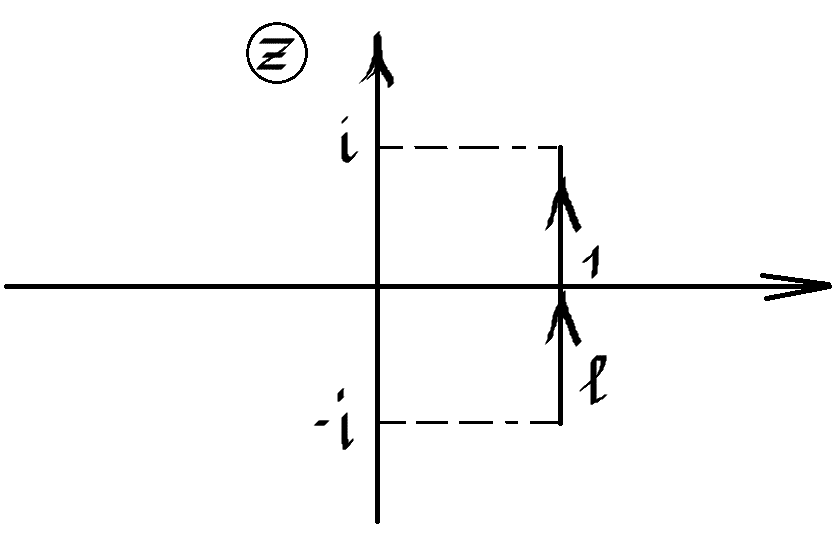
\includegraphics[height=0.3\textwidth]{lec30_1.png}}

Рассмотрим образ $L$ этого отрезка при 
$w = z^2 = (x + iy)^2 = x^2 - y^2 + 2ixy$

\begin{equation*}
    \begin{cases}
        u = Re\ w = x^2 - y^2\\
        v = Im\ w = 2xy
    \end{cases}
    L:
    \begin{cases}
        x = 1\\
        y|_{-1}^1
    \end{cases}
    \implies
    \begin{cases}
        u = 1 - y\\
        v = 2y|_{-2}^2
    \end{cases}
    \implies
    u = 1 - \frac{v^2}{4}, v|_{-2}^2 
\end{equation*}

\center{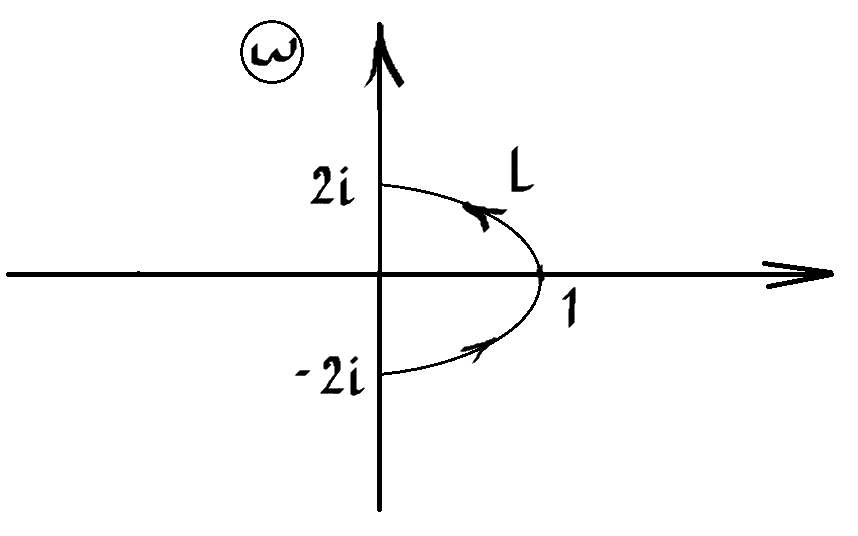
\includegraphics[height=0.3\textwidth]{lec30_2.png}}



\[\begin{gathered}
\text{Длина }L \stackrel{\eqref{lec30:1}}{=}
\left[
  \begin{array}{ccc}
     f^\prime\left(z\right) = \left(z^2\right) = 2z
  \end{array}
\right]
= \int\limits_l{2|z|\ |dz|} = 
\left[
  \begin{array}{ccc}
     z = 1 + iy\\
     y|_{-1}^1
  \end{array}
\right]
=  
\left[
  \begin{array}{ccc}
     |z| = \sqrt{1 + y^2}\\
     dz = idy \implies |dz| = dy
  \end{array}
\right]\\
= 2 \int\limits_{-1}^1{\sqrt{1 + y^2}\ dy} = 
4\int\limits_0^1{\sqrt{1 + y^2}\ dy} = 4
\left[
  \begin{array}{ccc}
     \sqrt{1 + y^2} + \ln(y + \sqrt{1 + y^2})
  \end{array}
\right]_0^1 = 
4(\sqrt{2} + \ln(1 + \sqrt{2}))
\end{gathered}\]


\item На комлексной плоскости рассмотрим квадрат D:
$\begin{cases}
    0 \leq x \leq 1,\\
    0 \leq y \leq 1;
\end{cases} w = z^2$

\center{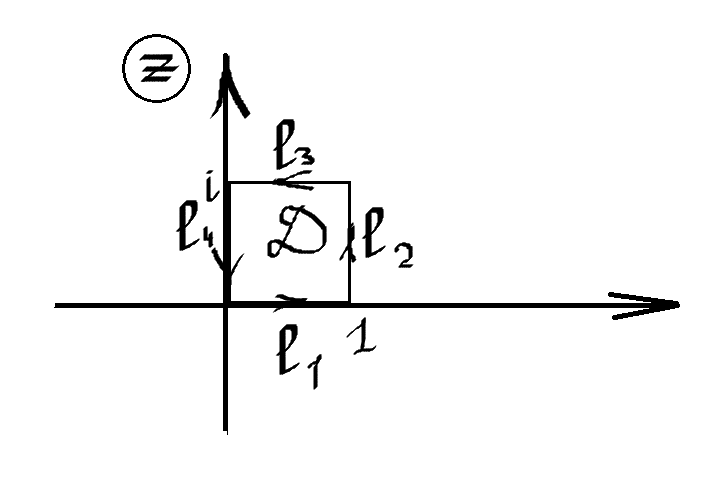
\includegraphics[height=0.3\textwidth]{lec30_3.png}}


\[\begin{gathered}
u = Re w = Re\ (x + iy)^2 = x^2 - y^2 \\
v = Im w = Im\ (x + iy)^2 = 2xy\\
    \text{a) }  l_1: y = 0,\ 0 \leq x \leq 1 \stackrel{w}{\implies}
L_1:
\begin{cases}
    u = x^2|_0^1\\
    v = 0
\end{cases}
\end{gathered}\]
\center{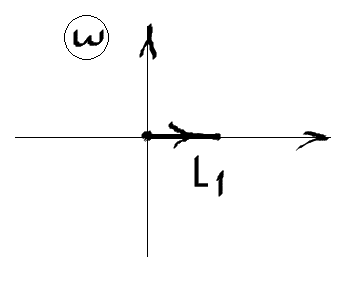
\includegraphics[height=0.3\textwidth]{lec30_4.png}}


\[
\text{б) } l_2: x = 1, 0 \leq x \leq 1 \stackrel{w}{\implies}
L_2: \begin{cases}
    u = 1 - y^2\\
    v = 2y|_0^2
\end{cases} \iff
\begin{cases}
    u = 1 - \frac{v^2}{4}\\
    v|_0^2
\end{cases}
\]
\center{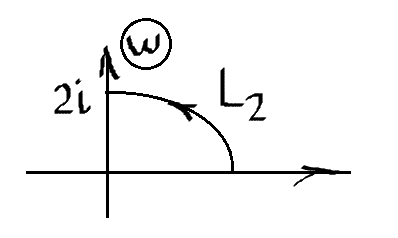
\includegraphics[height=0.3\textwidth]{lec30_5.png}}

\[
\text{в) } l_3: 
\begin{cases}
    y = 1\\
    x|_0^1
\end{cases} \implies
L_3:
\begin{cases}
    u = x^2 - 1\\
    v = 2x|_0^2
\end{cases} \iff
\begin{cases}
    u = \frac{v^2}{4} - 1\\
    v|_2^0
\end{cases}
\]
\center{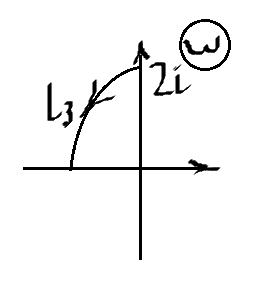
\includegraphics[height=0.3\textwidth]{lec30_6.png}}

\[
\text{г) } l_4:
\begin{cases}
    x = 0\\
    y|_0^1
\end{cases}
\stackrel{w}{\longrightarrow}
L_4:
\begin{cases}
    u = -y^2\ |_0^1\\
    v = 0
\end{cases}\]
\center{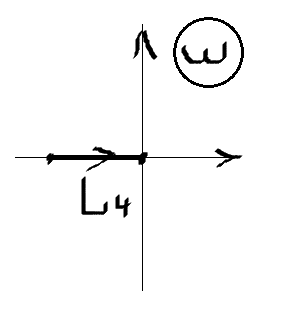
\includegraphics[height=0.3\textwidth]{lec30_7.png}}

\begin{flushleft}
  Имеем для L:
\end{flushleft}

\center{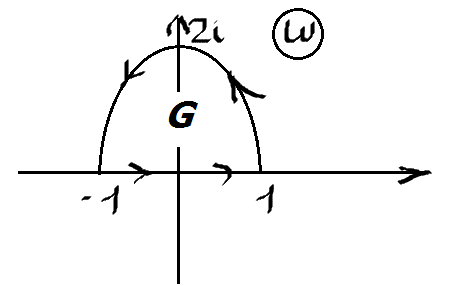
\includegraphics[height=0.3\textwidth]{lec30_8.png}}

\[\begin{gathered}
\text{пл. G} \stackrel{\eqref{lec30:2}}{=}  \left[
  \begin{array}{ccc}
     f^\prime\left(z\right) = 2z
  \end{array}
\right]
= \iint\limits_D{|2z|^2dxdy} = 4\iint\limits_D{\left(x^2 + y^2\right)\
dxdy} = \\
4\int\limits_0^1{dx}\int\limits_0^1{\left(x^2 + y^2\right) dy} = 
u\int\limits_0^1(x^2y + \frac{y^3}{3})\bigg|_{y=0}^{y=1}\ dx = 
4\int\limits_0^1{(x^2 + \frac{1}{3})\ dx} = 4(\frac{1}{3} + \frac{1}{3}) 
= \frac{8}{3}
\end{gathered}\]

\end{enumerate}
\end{examples}

\end{document}
